\documentclass[10pt, conference]{IEEEtran}
\usepackage[english]{babel}
\usepackage[usenames]{color}
\usepackage{colortbl}
\usepackage{comment}
\usepackage{graphicx}
\usepackage{xspace}
\usepackage{epsfig}
\usepackage{array, colortbl}
\usepackage{listings}
\usepackage{epstopdf}
\usepackage{multirow}
\usepackage{rotating}
%\usepackage{subfigure}
\usepackage{subfig}
\usepackage{float}
\usepackage[obeyspaces,hyphens,spaces]{url}
\usepackage{balance}
\usepackage{fancybox}
\usepackage{scalefnt}
\usepackage[normalem]{ulem}
%\pagestyle{plain}
\pagenumbering{arabic}
\pagestyle{empty}
\clubpenalty = 10000
\widowpenalty = 10000
\displaywidowpenalty = 10000
\usepackage{hyperref}
\usepackage{booktabs}
\usepackage{graphicx}
\usepackage[table,xcdraw]{xcolor}



% Keywords command
\providecommand{\keywords}[1]
{
  \small	
  \textbf{\textit{Keywords---}} #1
}


%New colors defined below
\definecolor{codegreen}{rgb}{0,0.6,0}
\definecolor{codegray}{rgb}{0.5,0.5,0.5}
\definecolor{codepurple}{rgb}{0.58,0,0.82}
\definecolor{backcolour}{rgb}{0.95,0.95,0.92}

%Code listing style named "mystyle"
\lstdefinestyle{mystyle}{
  backgroundcolor=\color{backcolour}, commentstyle=\color{codegreen},
  keywordstyle=\color{magenta},
  numberstyle=\tiny\color{codegray},
  stringstyle=\color{codepurple},
  basicstyle=\ttfamily\footnotesize,
  breakatwhitespace=false,
  breaklines=true,
  captionpos=b,
  keepspaces=true,
  numbers=left,
  numbersep=5pt,
  showspaces=false,
  showstringspaces=false,
  showtabs=false,
  tabsize=2
}

%"mystyle" code listing set
\lstset{style=mystyle}


\makeatletter
\renewcommand{\paragraph}[1]{\noindent\textsf{#1}.}
\newcommand{\etal}{et~al.\xspace}
\newcommand{\newtext}[1]{\textcolor{blue}{#1}}

% Reviewing commands
\newcommand{\Aurel}[1]{\textcolor{brown}{{\it [Aurel: #1]}}}
\newcommand{\todo}[1]{\textcolor{red}{\textbf{TODO: #1}}}


\newcommand{\add}[1]{\textcolor{red}{{\it $<$#1$>$}}}
\newcommand*{\RQOne}{ Is it possible to detect design smells in CNN deep learning programs based on modeling?}
\newcommand*{\RQTwo}{ What are the most prevalent design smells in CNN deep learning programs?}
\newcommand*{\RQThree}{ Are there any correlation between the program design smells?}



\title{Effective mutation test generation for End-to-End test programs using large language models}
% \author{Aurel Ikama$^{1}$, Foutse Khomh$^{1}$, Heng Li$^{1}$
%     \\
% \emph{$^{1}$ Dep. of Computer and Software Engineering, Polytechnique Montréal,
% Montréal}}
    

\author{Anonymous Author(s)}


\begin{document}
\maketitle

\begin{abstract}

\end{abstract}

\keywords{Mutation Testing, LLM, Software Engineering}



% Introduction
\section{Introduction}
\label{sec:introduction}

La qualité des applications web est une préoccupation majeure dans cycle de
vie d'un logiciel. Elle est souvent coûteuse et difficile à garantir. Elle
est par ailleurs cruciale pour les industries sensible comme la santé ou la
banque. Pour tester un logiciel on utilise entre des tests End-to-End (E2E). Ces tests sont généralement réalisés en utilisant des
frameworks tels que Selenium ou Cypress \cite{cerioli20205}. Les tests End-to-End (E2E) sont une approche de test qui vise à tester
le comportement d'une application web dans son ensemble selon la perspective de
l'utilisateur final. De ce fait, le programme sous test (PUT) est une boite
noire du point de vue du test. Cette caractéristique rends entre autres difficile
l'évaluation de la qualité des tests E2E tant pendant la création que la
maintenance du test. Ricca \etal \cite{ricca2019three} ont identifié plusieurs
défis liés à la qualité des tests E2E parmis lesquels on retrouve le problème de
la fragilité. Pour évaluer la fragilité des tests en général on utilise les tests de mutation \cite{hamimoune2016mutation}. Les tests de mutation est une
technique de test qui consiste à introduire des défauts dans le code source du
PUT pour évaluer la qualité des tests \cite{woodward1993mutation}. Cette méthode est utilisé dans
l'industrie pour les tests unitaires du fait de leur caractéristique de test en
boite blanche. Cependant quelques travaux commencent à s'intéresser à
l'application des tests de mutation pour les tests E2E. Yandrapally \etal
\cite{yandrapally2021mutation} propose dans le framework MaewU qui évalue des
suites de tests d'interface utilisateur (UI). Il introduit 16 opérations de mutation basées
sur 250 bug reports. Leotta \etal \cite{leotta2024mutta} propose par la suite l'outil
MUTTA qui permet d'automatiser le processus de test de mutation des tests E2E.
Ces travaux ont montré que les tests de mutation sont certes l'approche la plus
pertinante pour évaluer la qualité des tests E2E, mais il subsiste plusieurs défis
à relever. Parmi ces défis on retourve : (i) le coût élevé des tests de
mutation, (ii) l'identification et le filtre des mutants équivalents, et (iii)
l'éfficacité des tests de mutation. Dans ce travail, nous appliquons la génération des tests de mutation pour répondre à la problèmatique suivante : \textit{Comment optimiser la génération des tests de mutation pour les tests End-to-End (E2E) en surmontant les défis du coût élevé, de l’identification des mutants équivalents, et en maximisant l’efficacité des tests pour une évaluation fiable de la qualité des suites de tests ?}

Nous proposons une approche basée sur les modèles
de langage pour générer des tests de mutation plus réalistes, nécessaire et
diversifiés. Notre étude est conçue pour répondre aux questions de
recherche suivantes:

\begin{itemize}
    \item \textbf{RQ1:} LLM peut-il générer des tests de mutation plus efficaces que l'approche de pointe, en s'appuyant sur l'historique des erreurs

    \item \textbf{RQ2:} Quel est le modele de langage le plus adapté pour la génération des tests de mutation?

    \item \textbf{RQ3:} Peut-on identifier et réduire le nombre de mutants équivalents générés par notre approche?

    \item \textbf{RQ4:} Le coût (temps d'exécution et nombre de mutants) des tests de mutation générés par notre approche est-il réduit par rapport à l'approche de l'état de l'art?

\end{itemize}



% Background
\section{Background}
\label{sec:background}

\subsection{Mutant Generation}
A \textbf{mutant} is a small change in the source code of a PUT. The change is made to simulate a
real-life defect in the code \cite{offutt2001mutation, jia2010analysis}. The aim of mutation testing is to verify that a given test is capable of detecting the mutant by failing. This is known as killing the mutant. Mutants can be divided into two broad categories:

\begin{itemize}
    \item \textbf{Equivalent Mutants:} Mutants that do not affect the behavior of
          the PUT. These mutants are not useful for testing.
    \item \textbf{Non-Equivalent Mutants:} Mutants that affect the behavior of the PUT. These mutants are useful for testing.
\end{itemize}

Mutant generation is a crucial step in the mutation testing process. It is important to note that mutant generation can be either manual or automatic. Manual approaches obviously require human intervention. Whereas automatic approaches use tools such as PIT \cite{leotta2024mutta, coles2016pit}, Major \cite{just2014major},
Jumble \cite{irvine2007jumble} and Javalanche \cite{schuler2009javalanche}.
On the other hand, its tools can generate equivalent mutants, which can lead to incorrect results when evaluating mutation tests and therefore low efficiency. In a recent work, Leotta \etal \cite{leotta2024mutta} used PIT to generate mutants, as the tool provides the high number of mutators needed for E2E mutation testing.


\Aurel{ML in Mutation Testing}

\Aurel{LLM in Mutation Testing}
















% Study Design
\section{Methodology}
\label{sec:methodology}

In this section, we present our methodology to generate mutation tests for E2E
test programs. The methodology is illustrated in Figure \ref{fig:methodology}.
The methodology consists of the following steps:

\begin{itemize}
    
\item \textbf{Step 1:} \textit{Generating mutant:} We generate mutants with
adapted LLM models.
    
\item \textbf{Step 2:} \textit{Identifying equivalent mutants:} We use LLM
or graph methodology to identify equivalent mutants.
    
\item \textbf{Step 3:} \textit{Sorting mutants:} In this step we sort then
exclude equivalent mutants in the process. Exucluded equivalent mutants are
stored in a database for future mutant generation. We are inspired by the
Retrieval-augmented Generation (RAG)
methodology \Aurel{cite} to enrich LLM use in first step.
    
\item \textbf{Step 4:} \textit{Introducing generated mutant in PUT:} We
introduce the generated mutants in the PUT and check if PUT run successfully.

\item \textbf{Step 5:} \textit{Evaluating the generated mutants:} We evaluate
the generated mutants by checking if they are killed by the E2E test suite.
    \end{itemize}

\begin{figure}
  
    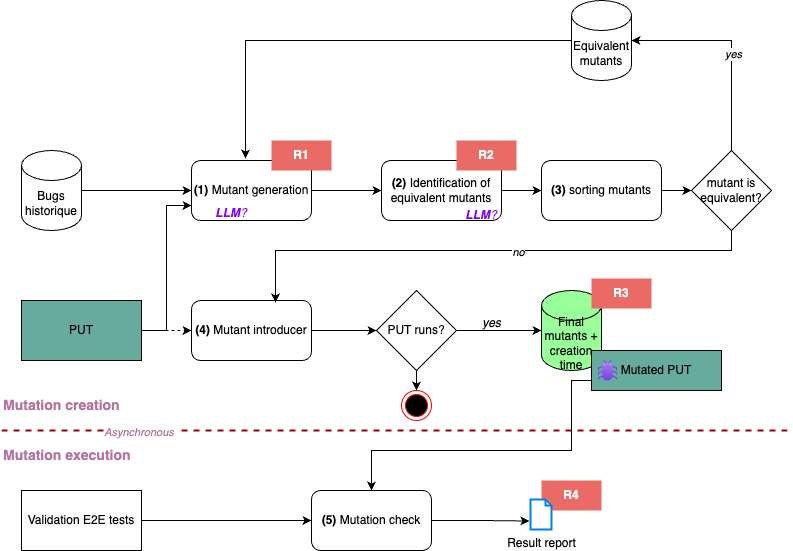
\includegraphics[width=0.5\textwidth]{figure/methodology.png}
    \caption{Methodology}
    \label{fig:methodology}
    
\end{figure}

% Data
\section{data}
\label{sec:data}


% Evaluation
\section{evaluation}
\label{sec:evaluation}


% Conclusion
\section{Conclusion}
\label{sec:conclusion}



\balance

\bibliographystyle{IEEEtran}
\bibliography{bibliography/citations}
\end{document}

